\section{问题分析}

四问要求的输出各不相同（两问要场分布、两问要时长），但支配现象的物理机制只有
一套：热量由热风经表面传入药材并向内部扩散，水分由内部扩散到表面后被气流带走。
因此本文先建立一个统一的一维轴对称耦合输运模型，再按各问指定的物性闭合与几何
条件逐层放开，四问共用同一份控制方程与同一套离散格式。图~\ref{fig:problem_relation}
给出四问的依赖关系：横向看是物性闭合从常物性到两套变物性的更替，纵向看是求解
诉求从给定时窗的场分布升级为阈值首达时刻，最后叠加求解域自身的收缩。

\begin{figure}[!htbp]
  \centering
  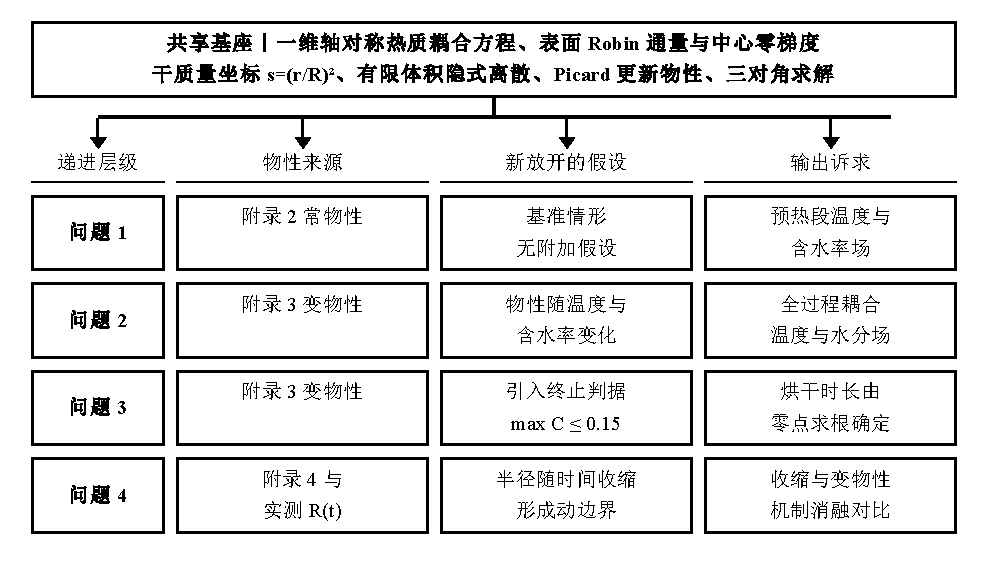
\includegraphics[width=0.9\textwidth,height=0.8\textheight,keepaspectratio]{../figures/fig_problem_relation_drawio.pdf}
  \caption{四问关系与递进层次}
  \label{fig:problem_relation}
\end{figure}

这一结构也决定了后文的写法：第~\ref{sec:model}~节把四问共用的守恒关系、
坐标变换与离散格式集中推导一次，此后每一问只交代它保留了什么、新增了什么、
结果因此改变了什么，不再重复整套方程。

\subsection{问题一的分析}

问题一要的是预热平衡阶段的两个场。判断模型维数不能只看几何：$L/R=12.5$ 说明
侧面传递远比端面重要，而题目要求的输出只按“到药材中心的距离”一个坐标索引——
若保留轴向坐标，同一半径不同高度处的温度并不相同，制表就没有唯一答案。
两条证据同时指向一维径向轴对称。

附录 2 的密度、比热容与热传导系数都是常数，只有水分扩散系数依赖含水率。
温度方程因此是线性的，可以用 Bessel 特征函数展开配合 Duhamel 叠加求出解析解；
含水率方程仍是非线性的，只能数值求解。这给出了一条难得的独立校验通道：
用解析解检验数值求解器在温度场上的正确性，再把同一套离散格式用于含水率场，
从而把“程序实现是否正确”与“物理建模是否恰当”分开验证。

表面换热强度需要先估计。热 Biot 数 $hR/k=1.3889$ 处于内外热阻相当的区间，
既不能把药材当作温度均匀的集中参数体，也不能把表面温度直接钉在热风温度上，
必须解偏微分方程并采用第三类边界条件。传质一侧的量级更悬殊：初始含水率下
扩散系数约 $4.94\times10^{-9}$ m$^2$/s，对应的质 Biot 数约 $3.24$。
两个方向的阻力都不可忽略。

一个需要提前判定的取舍是汽化潜热。附录未给出汽化潜热数值，若在温度边界条件中
补入蒸发冷却项并按常见量级 $2.4\times10^6$ J/kg 估算，$1800$ s 时蒸发耗热约
$655$ W/m$^2$，而同期对流供热仅约 $118$ W/m$^2$，净热流为负、药材应当降温，
与附件 1 给出的升温工况和“预热”这一名称直接矛盾。故本题的既定语义是热、
质两个通道分别按对流规律传递，不引入潜热耦合项。

\subsection{问题二的分析}

问题二把时间窗从预热段拉长到整个烘干过程，并明确要求经验公式统一采用附录 3。
“统一”二字排除了按阶段切换物性的做法：即使在 $t\le1800$ s 的预热段，
也应使用附录 3 而非附录 2。由此产生一个必须显式说明的现象——问题二在
$1800$ s 处给出的数值与问题一并不相同。这不是前后矛盾，而是两问采用了不同的
物性闭合，若不说明，容易被误读为计算不自洽。

附录 3 只重新给出了密度、比热容、热传导系数与扩散系数，没有重新给出对流换热
系数与对流传质系数，故这两个表面系数沿用附录 2 的取值，这是不引入任何自由参数的
唯一读法。附录 3 的三个物性都写成湿基含水率 $C/(C+1)$ 的线性函数，
初始状态下该组合等于 $0.7183$；若误把它简化为干基含水率 $C$，热传导系数会被
放大两倍以上。扩散系数中的 $\mathrm{e}^{-3850/T}$ 属于 Arrhenius 型，
指数上的 $3850$ 已经含有活化能与气体常数之比，温度必须用热力学温标；
误用摄氏温标会使扩散系数偏离数十个数量级。

附件 1 只覆盖到 $14400$ s，而全过程需要几十小时，故必须约定此后的烘房条件。
附件 1 末段已进入平台，采用末 $24$ 个数据点的均值作为恒温干燥段的取值既符合
“恒温干燥”的字面含义，也有数据支撑，且比取单点更能抑制测量波动。
这一约定支配了后两问绝大部分时间轴，其影响必须与结果一同披露。

\subsection{问题三的分析}

问题三新增的内容只有终止判据。“各处的水分浓度应低于 $0.15$ kg/kg”是一个
作用在空间最大值上的条件，而不是作用在截面平均值上的条件。这一区分在本题
量级很大：本文实际算得的平均含水率在 $36$ h 就已降到 $0.1499$，若误用均值判据
会得到约 $36$ h 的答案，比逐点判据短三成以上，而此时中心处仍有 $0.1858$ kg/kg，
药材内部远未达标。

含水率剖面沿半径单调递减这一性质使空间最大值取于中心，于是场判据可化为
一个标量判据，阈值首达时刻用相邻输出步之间的插值定位。判据能否在有限时间内达到也需要
检验：表面处的驱动浓度由空气含湿量给出，其平台值约 $0.05$ kg/kg，低于阈值
$0.15$ kg/kg，故存在有限的达标时刻。题面“一般持续 $2$ 至 $3$ 天”给出了一个
独立于模型之外的量级区间，可用来反查答案是否落在合理范围。

\subsection{问题四的分析}

问题四相对问题三只增加两件事：物性闭合换成附录 4，半径由固定值改为附件 2 给出的
实测时程。“请根据附件 2”意味着收缩是给定的运动学数据，不是待求量，
因此模型不需要补充任何收缩本构，也不应由含水率反推半径。附件 2 显示半径从
$2.000$ cm 单调降到 $1.198$ cm，横截面积仅剩三分之一略多，而全部收缩量的
$78.1\%$ 发生在前 $6$ h，正是传质最活跃的时段，扩散路程在最关键的阶段被大幅缩短。

两个新增因素的作用方向相反：附录 4 在初始状态下给出的扩散系数比附录 3 小 $5.4$ 倍，
使干燥变慢；收缩缩短扩散路程，使干燥变快。若只比较问题三与问题四的总时长，
净变化不大，很容易得出“收缩影响有限”的错误判断。因此必须做四组合的消融实验，
把两个机制分别量化，再检查两者能否线性叠加。

附件 2 的收缩数据与附录 4 的密度公式还存在一处不自洽：若认为整根药材的质量
由附录 4 的密度式描述，则由实测半径反演出的平均含水率会在若干小时后变成负值。
这一矛盾无法在题设范围内消除，但可以如实披露，并说明为什么仍以附件 2 的实测
半径为准。
